
\subsection*{Calidad de los estimadores del centro de simetría}

En esta parte se compara el comportamiento de los tres estimadores del centro de simetría considerados en el proyecto: el estimador por minimización \(\hat\theta_{\min}\), la mediana \(\hat\theta_{\mathrm{med}}\) y la media afeitada \(\hat\theta_\alpha\). La comparación se divide en dos escenarios. Bajo \(H_0\), como la distribución sí es simétrica y el centro verdadero es conocido, se evalúa la precisión de cada estimador mediante RMSE, MAE, sesgo y distribución del error. Bajo \(H_a\), en cambio, no existe un centro verdadero de simetría; por tanto, solo se analiza la estabilidad de los estimadores a través de la variabilidad de \(\hat\theta\) entre réplicas.

\subsubsection*{Precisión bajo \texorpdfstring{$H_0$}{H0}: RMSE, MAE y sesgo}

Para evaluar directamente la calidad de los estimadores bajo \(H_0\), se consideran las dos distribuciones simétricas usadas en las simulaciones: Cauchy\((2,1)\) y Uniforme\((1,3)\). En ambos casos el centro verdadero es \(\theta=2\), por lo que se reportan el RMSE, el MAE y el sesgo empírico de cada estimador.


\begin{figure}[H]
  \centering
  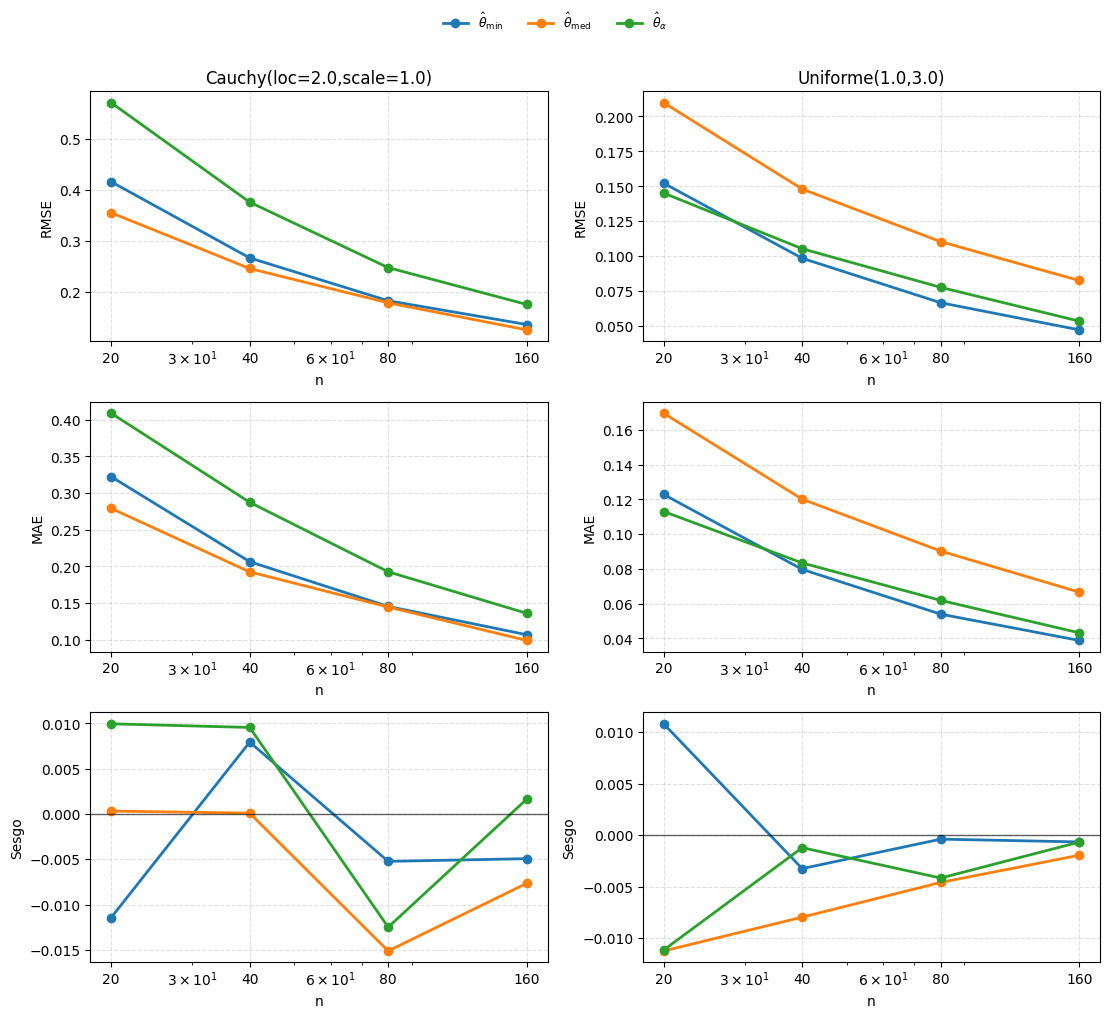
\includegraphics[width=\textwidth]{../results/figures/discusion/theta_estimators_h0_all_metrics.png}
  \caption{Comparación de los estimadores del centro bajo \(H_0\). Se muestran RMSE, MAE y sesgo para Cauchy\((2,1)\) y Uniforme\((1,3)\), usando \(n\in\{20,40,80,160\}\).}
  \label{fig:theta-estimators-h0}
\end{figure}

En la distribución Cauchy, la mediana presenta el mejor comportamiento global en RMSE y MAE para todos los tamaños muestrales. Esto es consistente con la robustez de la mediana frente a colas pesadas. El estimador \(\hat\theta_{\min}\) mejora al aumentar \(n\) y se acerca mucho a la mediana para \(n=80\) y \(n=160\), mientras que la media afeitada muestra errores mayores, especialmente para muestras pequeñas.

En la distribución Uniforme, el patrón cambia: \(\hat\theta_{\min}\) tiene el menor RMSE y MAE para \(n\ge 40\), mientras que la media afeitada es competitiva para \(n=20\). La mediana resulta menos eficiente en este caso, con errores sistemáticamente mayores. Esto sugiere que, en distribuciones simétricas de soporte acotado, el estimador por minimización aprovecha mejor la estructura global de la muestra.

El sesgo empírico es pequeño para los tres estimadores y tiende a cero al crecer \(n\). Por tanto, las diferencias principales entre ellos no se deben a sesgo sistemático, sino a varianza y sensibilidad frente a colas pesadas. En conjunto, \(\hat\theta_{\min}\) es el estimador más competitivo bajo soporte acotado, mientras que la mediana es preferible cuando hay colas pesadas.

\subsubsection*{Distribución de los errores de estimación bajo \texorpdfstring{$H_0$}{H0}}

Para complementar las métricas anteriores, se analiza la distribución completa de los errores \(\hat\theta-\theta\). Esto permite observar no solo el error promedio, sino también la dispersión y la estabilidad de cada estimador.


\begin{figure}[H]
  \centering
  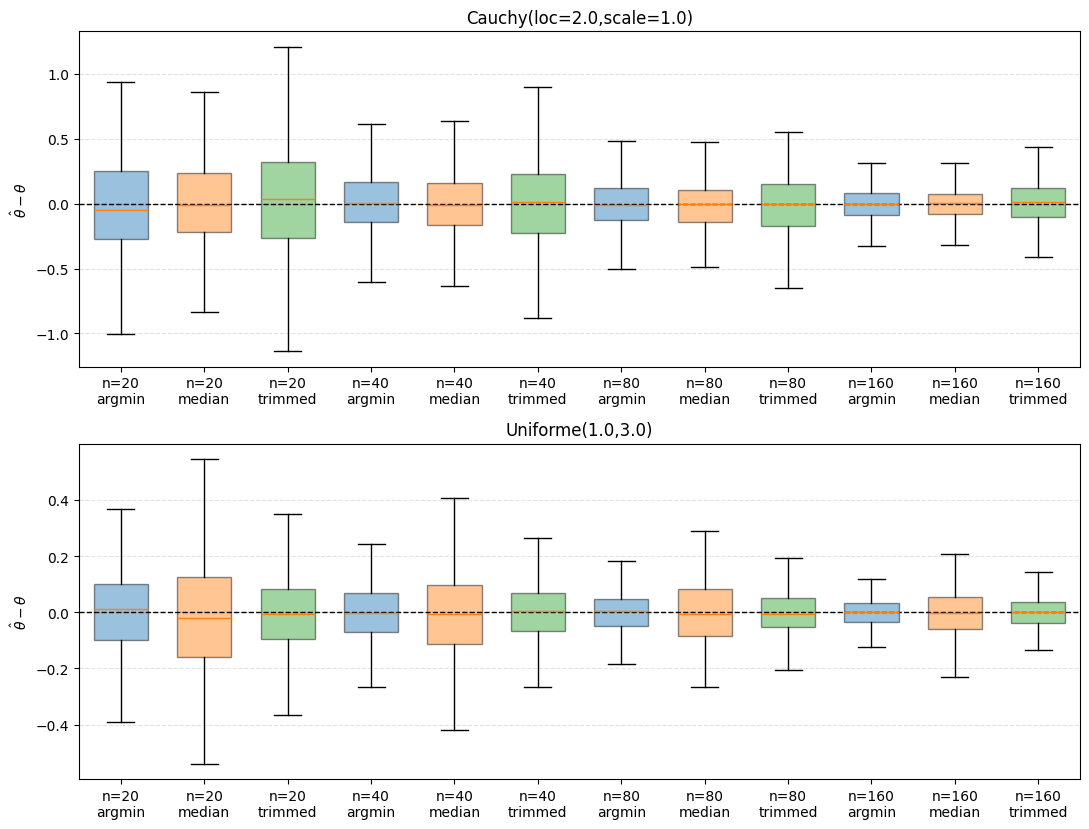
\includegraphics[width=\textwidth]{../results/figures/discusion/theta_estimator_error_boxplots_h0.png}
  \caption{Distribución de los errores de estimación \(\hat\theta-\theta\) bajo \(H_0\), para Cauchy\((2,1)\) y Uniforme\((1,3)\). Se muestran diagramas de caja para \(\hat\theta_{\min}\), la mediana y la media afeitada, en \(n\in\{20,40,80,160\}\).}
  \label{fig:theta-error-boxplots-h0}
\end{figure}

La Figura~\ref{fig:theta-error-boxplots-h0} confirma las conclusiones anteriores. En ambos modelos, la dispersión de \(\hat\theta-\theta\) disminuye al aumentar \(n\), como es esperable por consistencia. Sin embargo, la forma en que se concentra la distribución del error depende del estimador y de la distribución subyacente.

Bajo Cauchy, la mediana presenta cajas más estrechas y centradas alrededor de \(0\) que los otros estimadores, especialmente para \(n=20\) y \(n=40\), lo que refuerza su mayor estabilidad en presencia de colas pesadas. El estimador \(\hat\theta_{\min}\) también mejora con \(n\), pero exhibe una dispersión algo mayor en muestras pequeñas. La media afeitada es la más variable, en concordancia con sus mayores valores de RMSE y MAE.

Bajo Uniforme, en cambio, \(\hat\theta_{\min}\) y la media afeitada muestran una dispersión menor que la mediana para \(n\ge 40\). En particular, \(\hat\theta_{\min}\) exhibe cajas más compactas para \(n=80\) y \(n=160\), lo que explica su ventaja en RMSE y MAE en esta distribución. La mediana conserva un sesgo pequeño, pero su variabilidad es mayor de forma sistemática.

En conjunto, los diagramas de caja muestran que las diferencias entre estimadores provienen principalmente de la variabilidad de \(\hat\theta\), más que de sesgos apreciables. Esto respalda la conclusión de que la mediana es preferible bajo colas pesadas, mientras que \(\hat\theta_{\min}\) resulta más eficiente en distribuciones simétricas de soporte acotado.


\subsubsection*{Estabilidad bajo \texorpdfstring{$H_a$}{Ha}}

Bajo \(H_a\), las distribuciones consideradas no son simétricas; por tanto, no existe un verdadero centro de simetría contra el cual comparar los estimadores. En este caso, no se calculan RMSE ni sesgo respecto a un parámetro real. En su lugar, se analiza la estabilidad de \(\hat\theta\), medida por su desviación estándar entre réplicas de Monte Carlo.


\begin{figure}[H]
  \centering
  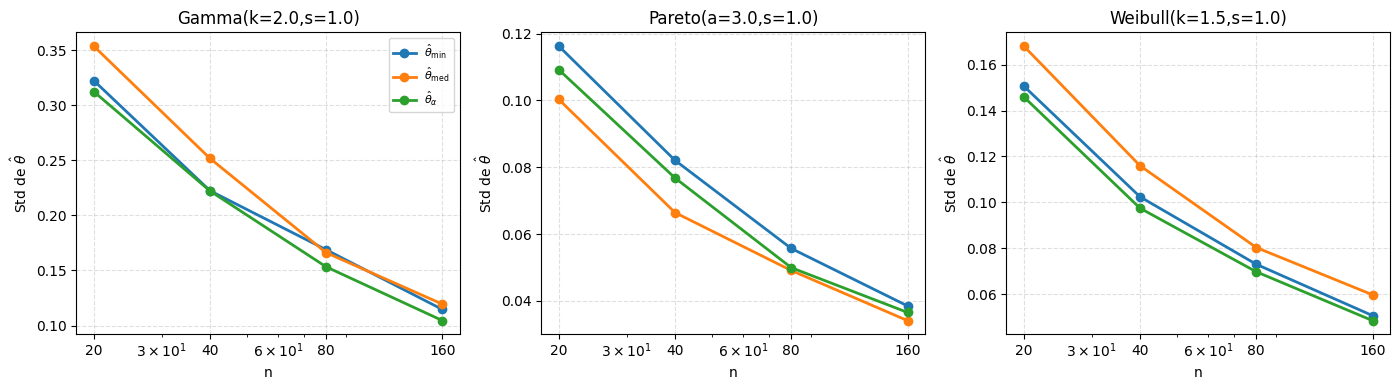
\includegraphics[width=\textwidth]{../results/figures/discusion/theta_estimator_std_ha.png}
  \caption{Desviación estándar de \(\hat\theta\) bajo \(H_a\), para las distribuciones Gamma\((2,1)\), Pareto\((3,1)\) y Weibull\((1.5,1)\).}
  \label{fig:theta-std-ha}
\end{figure}

Bajo \(H_a\) no existe un verdadero centro de simetría, por lo que ya no tiene sentido comparar los estimadores mediante RMSE o sesgo respecto a un parámetro real. En este caso, el interés se desplaza hacia la estabilidad de \(\hat\theta\), medida aquí por su desviación estándar a través de las réplicas de Monte Carlo.

La Figura~\ref{fig:theta-std-ha} muestra que la variabilidad de los tres estimadores disminuye con \(n\) en las tres distribuciones asimétricas consideradas. Sin embargo, el orden relativo entre ellos depende de la forma de la distribución. En Gamma y Weibull, la media afeitada \(\hat\theta_\alpha\) es la más estable en casi todos los tamaños muestrales, seguida muy de cerca por \(\hat\theta_{\min}\), mientras que la mediana presenta mayor dispersión. En cambio, bajo Pareto, la mediana resulta ser el estimador más estable para todos los \(n\), lo cual es coherente con su mayor robustez frente a colas pesadas.

En conjunto, estos resultados sugieren que, fuera de la hipótesis de simetría, la elección del estimador depende en buena medida de la severidad de la asimetría y del peso de las colas. La media afeitada ofrece la mejor estabilidad en alternativas moderadamente asimétricas como Gamma y Weibull, mientras que la mediana vuelve a destacar cuando la asimetría viene acompañada de colas más pesadas, como en Pareto.




Se evalúan los tres estimadores del centro usados en las pruebas bootstrap,
ahora como estimadores puntuales de la localización ($R=500$ réplicas Monte Carlo
por combinación distribución $\times$ $n$):

\begin{enumerate}
  \item $\hat\theta_{\min}$ \textbf{(argmin de $T_n$, Schuster-Narvarte)}: minimizador exacto de $T_n(\theta)$ obtenido por el algoritmo combinatorio de Schuster-Narvarte.
  \item $\hat\theta_{\mathrm{med}}$ \textbf{(mediana muestral)}: minimiza $\sum_i|X_i-\theta|$. Máxima robustez (breakdown $50\%$), asintóticamente eficiente para distribuciones de Cauchy.
  \item $\hat\theta_\alpha$ \textbf{(media afeitada $10\%$)}: media de los datos sin el $10\%$ extremo en cada cola.
\end{enumerate}

% -----------------------------------------------------------
\subsubsection*{Bajo \texorpdfstring{$H_0$}{H0}: sesgo y RMSE}

\begin{figure}[H]
  \centering
  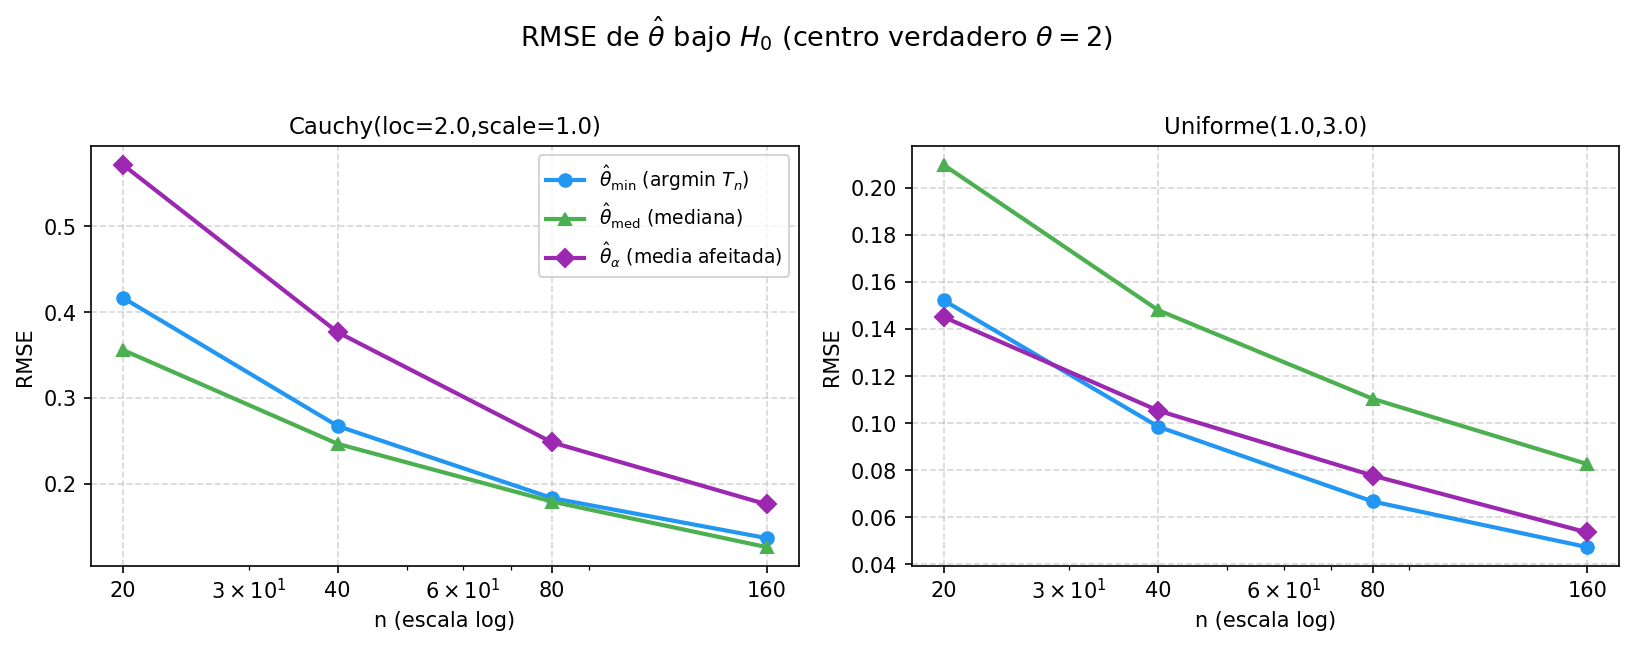
\includegraphics[width=\textwidth]{../results/figures/apendice_rmse_h0.png}
  \caption{
    \textbf{RMSE} de los tres estimadores bajo $H_0$ en función de $n$ (escala log).
    Izquierda: Cauchy$(2,1)$ (colas pesadas); derecha: Uniforme$(1,3)$ (colas ligeras).
    El centro verdadero es $\theta=2$ en ambos casos.
  }
  \label{fig:apendice-rmse-h0}
\end{figure}

Los patrones de RMSE difieren según la distribución nula:

\begin{itemize}
  \item \textbf{Cauchy$(2,1)$} (Figura~\ref{fig:apendice-rmse-h0}, izquierda).
    La mediana es el estimador con menor RMSE en todos los $n$ (es el estimador de máxima verosimilitud de la Cauchy). El argmin ocupa el segundo lugar. La media afeitada presenta el mayor RMSE, pues no es eficiente bajo colas tan pesadas: para $n=20$ su RMSE es $0.572$, frente a $0.356$ de la mediana.

  \item \textbf{Uniforme$(1,3)$} (Figura~\ref{fig:apendice-rmse-h0}, derecha).
    El orden se invierte: la media afeitada y el argmin tienen los menores RMSE (virtualmente iguales para $n\ge40$), mientras que la mediana tiene el \emph{mayor} RMSE. Para $n=160$: argmin~$0.047$, media afeitada~$0.054$, mediana~$0.083$. Esto se explica porque para la Uniforme, cuya densidad es constante, la media de la muestra transporta más información sobre el centro que la observación mediana; la media afeitada captura esto parcialmente, y el argmin la explota completamente al integrar todos los pares de Walsh.
\end{itemize}

\begin{figure}[H]
  \centering
  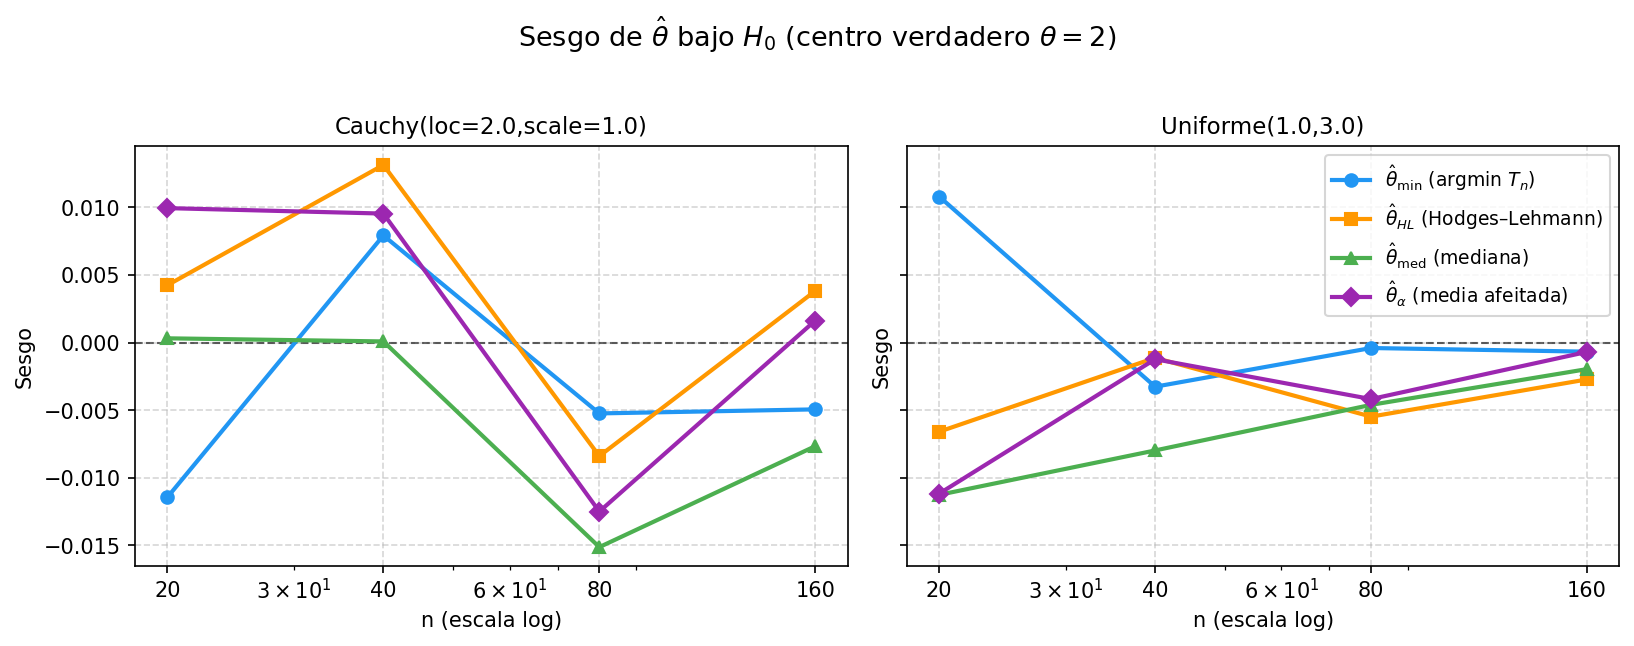
\includegraphics[width=\textwidth]{../results/figures/apendice_bias_h0.png}
  \caption{
    \textbf{Sesgo} de los tres estimadores bajo $H_0$ ($\theta=2$) en función de $n$.
    La línea punteada marca sesgo cero. Las desviaciones respecto a cero son
    estadísticamente indistinguibles de cero ($R=500$, $\mathrm{SE}\approx\mathrm{RMSE}/\sqrt{500}$).
  }
  \label{fig:apendice-bias-h0}
\end{figure}

Como muestra la Figura~\ref{fig:apendice-bias-h0}, los tres estimadores son prácticamente insesgados bajo $H_0$ ($|\text{sesgo}|<0.015$ en todos los casos). Este resultado confirma que el conservatismo del test $T_n$ con estimador argmin no proviene de un sesgo en la estimación de $\theta$, sino de que minimizar $T_n$ sobre los datos observados reduce directamente el estadístico.

\begin{figure}[H]
  \centering
  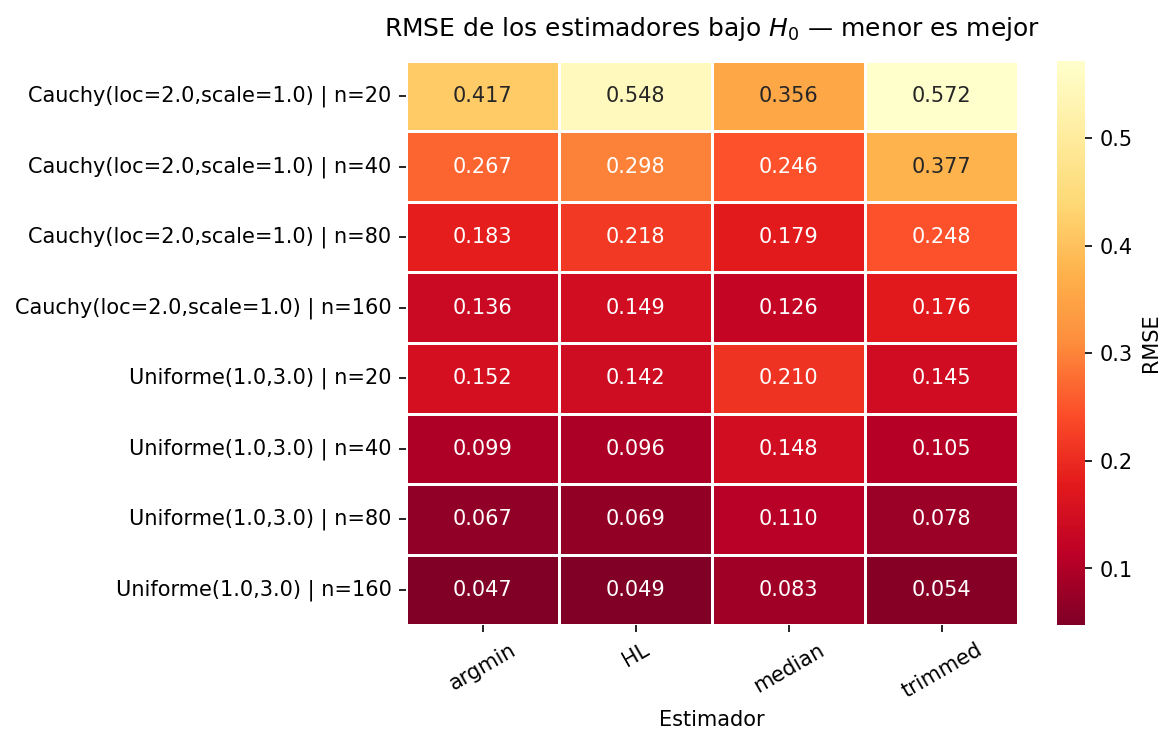
\includegraphics[width=\textwidth]{../results/figures/apendice_rmse_heatmap.png}
  \caption{
    \textbf{Heatmap de RMSE} bajo $H_0$: tonos más claros indican menor RMSE (mejor estimador).
    El argmin domina bajo Uniforme; la mediana domina bajo Cauchy.
  }
  \label{fig:apendice-rmse-heatmap}
\end{figure}

% -----------------------------------------------------------
\subsubsection*{Bajo \texorpdfstring{$H_a$}{Ha}: distribución de \texorpdfstring{$\hat\theta$}{theta hat}}

Bajo las distribuciones alternativas (Gamma, Weibull, Pareto) no existe un centro de simetría verdadero; se estudia dónde ``localiza'' cada estimador.

\begin{figure}[H]
  \centering
  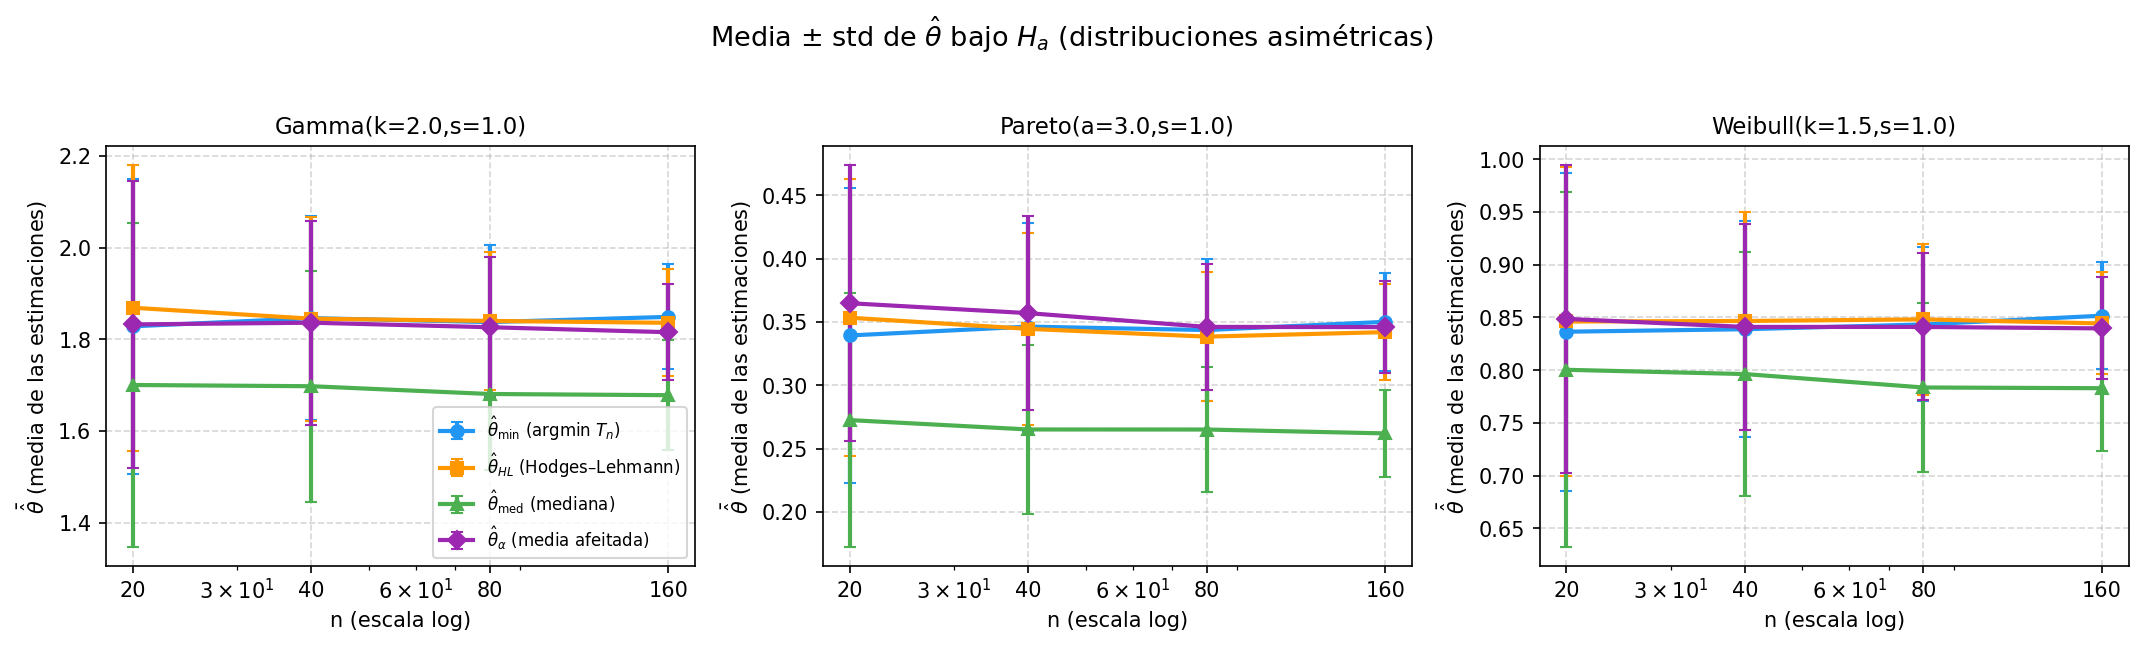
\includegraphics[width=\textwidth]{../results/figures/apendice_theta_ha.png}
  \caption{
    \textbf{Media $\pm$ desviación estándar} de $\hat\theta$ bajo $H_a$:
    Gamma$(2,1)$ (izquierda), Weibull$(1.5,1)$ (centro) y Pareto$(3,1)$ (derecha).
    La distribución de $\hat\theta$ converge con $n$ hacia un valor determinístico
    específico de cada estimador.
  }
  \label{fig:apendice-theta-ha}
\end{figure}

Las diferencias entre estimadores son más pronunciadas bajo $H_a$:

\begin{itemize}
  \item \textbf{Mediana ($\hat\theta_{\mathrm{med}}$)}: converge al cuantil $0.5$ de la distribución asimétrica.
    Para Gamma$(2,1)$: $\bar{\hat\theta}\approx 1.68$ (cuantil $0.5$ teórico $\approx 1.68$); para Pareto$(3,1)$: $\bar{\hat\theta}\approx 0.26$.

  \item \textbf{Argmin ($\hat\theta_{\min}$)}: localiza el centro en un punto intermedio entre la mediana y la media de la distribución. Para Gamma$(2,1)$: $\bar{\hat\theta}\approx 1.84$; para Pareto$(3,1)$: $\bar{\hat\theta}\approx 0.35$. Este desplazamiento positivo respecto a la mediana es propio de un estimador que promedia pares (Walsh averages): bajo asimetría derecha, hay más pares con suma elevada que baja, desplazando el argmin hacia arriba.

  \item \textbf{Media afeitada}: perfil muy similar al argmin ($\bar{\hat\theta}\approx 1.82$--$1.84$ para Gamma), con ligera ventaja en varianza para $n$ grande.

  \item \textbf{Variabilidad}: la desviación estándar decrece como $\mathcal{O}(n^{-1/2})$ en los tres estimadores; no hay diferencias apreciables de dispersión entre ellos para $n\ge 40$.
\end{itemize}

La diferencia en la localización de $\hat\theta$ entre la mediana y los demás estimadores es relevante para la potencia del test: el argmin ubica el centro en un punto que hace la distribución empírica ``más alejada'' de su simetrización, de modo que $T_n(\hat\theta_{\min})$ resulta comparativamente mayor bajo $H_a$ que $T_n(\hat\theta_{\mathrm{med}})$. El bootstrap calibra este efecto correctamente (también minimiza sobre cada remuestra), y el resultado neto es la mayor potencia del argmin observada en la Sección~\ref{sec:potencia}.
